\documentclass{article} % For LaTeX2e
\usepackage{nips10submit_e,times}
%\documentstyle[nips10submit_09,times,art10]{article} % For LaTeX 2.09
\usepackage[numbers]{natbib}

\usepackage{fullpage}
\usepackage{amssymb}
\usepackage{amsfonts}
\usepackage{amsmath}
\usepackage{stmaryrd}
\usepackage{url}
\usepackage{graphicx}
\usepackage{subfig}
\usepackage{alltt}
\usepackage{color}
\usepackage{soul}
\usepackage{wrapfig}
\usepackage{array}
\usepackage[all]{xy}
\usepackage[]{algorithm2e}
\usepackage{pdfpages}
\usepackage[mathscr]{euscript} % e.g. \mathscr{R}
%\usepackage{mathrsfs} % e.g. \mathscr{R}

%\usepackage{setspace}

\DeclareMathOperator*{\argmax}{arg\!\,max}
\newcommand{\mc}[1]{\mathcal{#1}}
\newcommand{\mb}[1]{\mathbb{#1}}
\newcommand{\norm}[1]{\ensuremath{\lVert{#1}\rVert}}
\newcommand{\?}{\stackrel{?}{=}}
\newcommand{\deltaeq}{\stackrel{\Delta}{=}}

\usepackage{tikz}
\usetikzlibrary{arrows,decorations.pathmorphing,backgrounds,positioning,fit,petri}

%\title{Mixture of Plackett-Luce (PL) Models for Rank Data}

%\author{
%Shubhomoy Das
%}


% The \author macro works with any number of authors. There are two commands
% used to separate the names and addresses of multiple authors: \And and \AND.
%
% Using \And between authors leaves it to \LaTeX{} to determine where to break
% the lines. Using \AND forces a linebreak at that point. So, if \LaTeX{}
% puts 3 of 4 authors names on the first line, and the last on the second
% line, try using \AND instead of \And before the third author name.

\newcommand{\fix}{\marginpar{FIX}}
\newcommand{\new}{\marginpar{NEW}}
\newcommand{\horrule}[1]{\rule{\linewidth}{#1}} % Create horizontal rule command
\nipsfinalcopy % Uncomment for camera-ready version

\normalsize

\begin{document}

\begin{center}
\horrule{0.5pt} \\[0.4cm] % Thin top horizontal rule
\LARGE Parameter Estimation of Polya's Distribution\\
\vspace{5pt}
\large Md Amran Siddiqui \normalsize and \large Tadesse Zemicheal\\
\vspace{5pt}
\horrule{2pt} % Thick bottom horizontal rule
\end{center}
%\maketitle

%\begin{abstract}
% Abstract
%\end{abstract}

%\pagebreak

\section{Introduction} \label{INTRO}
In this project our goal is to estimate parameters of Poly's distribuiotn using different methods like maximum likelihood and method of moments, and compare their performance with the Cramer Rao Lower bound. In Polya distribution we have $k$ parameters $p_1, p_2, ..., p_k$ for multinomial distribution representing probabilities for $k$ categories. These $k$ parameters are random and coming from Dirichlet distribution with parameters $\alpha_1, \alpha_2, ..., \alpha_k$. In this project we explore a simple case where number of categories are just two. Hence, the multinomial reduces to Binomial and Dirichlet reduces to Beta distribution.

\section{Cramer Rao Lower Bound}\label{CRLB}
The probability mass function for Polya distributin is:

\begin{align}
p(x\ |\ \alpha) &=  
\frac{n!}{\prod\limits_{k} n_{k!}}
\frac{\Gamma(\sum\limits_{k}\alpha_k)}{\Gamma(n+\sum\limits_{k}\alpha_k)}
\prod\limits_{k}\frac{\Gamma(n_{k} + \alpha_k)} {\Gamma(\alpha_k)}\label{pdf}
\end{align}

where,\\
the parameter vector is:
$\theta=\left[\begin{matrix}
\alpha_1\\
\alpha_2\\
.\\
.\\
\alpha_k
\end{matrix}\right]$\\
$n = n(x) = $ length of a data sample $x$\\
$n_{k} = n_k(x) = $ number of k category elements in $x$\\

Now, for $m$ observations $x_1, x_2, ..., x_m$

\begin{align}
p(x_1,x_2, ..., x_m\ |\ \alpha) &= \prod_{i=1}^{m}{\left( 
\frac{n_i!}{\prod_{k} n_{ik!}} 
\frac{\Gamma(\sum_{k}\alpha_k)}{\Gamma(n_i+\sum_{k}\alpha_k)}
\prod_{k}\frac{\Gamma(n_{ik} + \alpha_k)} {\Gamma(\alpha_k)}
\right)  }
\end{align}

The log likelihood is:

\begin{align}
& log\ p(x_1,x_2, ..., x_m\ |\ \alpha) \\
&= \sum_{i=1}^{m}log{\left( 
\frac{n_i!}{\prod_{k} n_{ik}!}
\frac{\Gamma(\sum_{k}\alpha_k)}{\Gamma(n_i+\sum_{k}\alpha_k)}
\prod_{k}\frac{\Gamma(n_{ik} + \alpha_k)} {\Gamma(\alpha_k)}
\right)  }\\
&= \sum_{i=1}^{m}{\left( log(n_i!) - \sum_{k}log(n_{ik}!)! + log(\Gamma(\sum_{k}\alpha_k))
- log(\Gamma(n_i+\sum_{k}\alpha_k)) + \sum_{k} log(\Gamma(n_{ik} + \alpha_k)) - \sum_{k} log(\Gamma(\alpha_k)) \right)}
\end{align}

Differentiating in terms of $\alpha_k$:
\begin{align}
\frac{d\ log\ p(D\ |\ \alpha)}{d\ \alpha_k} &= 
\sum_{i=1}^{m} \left({ \psi(\sum_{k}\alpha_k) - \psi(n_i+\sum_{k}\alpha_k) + \psi(n_{ik} + \alpha_k) - \psi(\alpha_k) }\right)\\
\frac{d^2\ log\ p(D\ |\ \alpha)}{d\ \alpha_k^2} &= 
\sum_{i=1}^{m} \left({ \psi'(\sum_{k}\alpha_k) - \psi'(n_i+\sum_{k}\alpha_k) + \psi'(n_{ik} + \alpha_k) - \psi'(\alpha_k) }\right)\\
\frac{d^2\ log\ p(D\ |\ \alpha)}{d\ \alpha_k\ d\ \alpha_j} &= 
\sum_{i=1}^{m} \left({ \psi'(\sum_{k}\alpha_k) - \psi'(n_i+\sum_{k}\alpha_k) }\right)
\end{align}

Now, for beta binomial case (k = 2), we have two parameters $\alpha_1$ and $\alpha_2$. Hence the FIM is:


\begin{align}
FIM = -E\left[\begin{matrix}
  \frac{d^2\ log\ p(D\ |\ \alpha)}{d\ \alpha_1^2} & \frac{d^2\ log\ p(D\ |\ \alpha)}{d\ \alpha_1\ d\ \alpha_2}\\
  \frac{d^2\ log\ p(D\ |\ \alpha)}{d\ \alpha_2\ d\ \alpha_1} & \frac{d^2\ log\ p(D\ |\ \alpha)}{d\ \alpha_2^2}
 \end{matrix}\right]
\end{align}

\begin{align}
\left[\begin{matrix}
  \sum\limits_{i=1}^{m} \left({ \psi'(\sum\limits_{k}\alpha_k) - \psi'(n_i+\sum\limits_{k}\alpha_k) + \psi'(n_{i1} + \alpha_1) - \psi'(\alpha_1) }\right) & \sum\limits_{i=1}^{m} \left({ \psi'(\sum\limits_{k}\alpha_k) - \psi'(n_i+\sum\limits_{k}\alpha_k) }\right)\\
  \sum\limits_{i=1}^{m} \left({ \psi'(\sum\limits_{k}\alpha_k) - \psi'(n_i+\sum\limits_{k}\alpha_k) }\right) & \sum\limits_{i=1}^{m} \left({ \psi'(\sum\limits_{k}\alpha_k) - \psi'(n_i+\sum\limits_{k}\alpha_k) + \psi'(n_{i2} + \alpha_2) - \psi'(\alpha_2) }\right)
 \end{matrix}\right]
\end{align}

\begin{align}
FIM_{11} &= -E\left[\sum\limits_{i=1}^{m} \left({ \psi'(\sum\limits_{k}\alpha_k) - \psi'(n_i+\sum\limits_{k}\alpha_k) + \psi'(n_{i1} + \alpha_1) - \psi'(\alpha_1) }\right)\right]\\
&= -\sum\limits_{i=1}^{m} \left({ \psi'(\sum\limits_{k}\alpha_k) - \psi'(n_i+\sum\limits_{k}\alpha_k) + E\left[\psi'(n_{i1} + \alpha_1)\right] - \psi'(\alpha_1) }\right)\\
&= -m * \left({ \psi'(\sum\limits_{k}\alpha_k) - \psi'(n_i+\sum\limits_{k}\alpha_k) + E\left[\psi'(n_{i1} + \alpha_1)\right] - \psi'(\alpha_1) }\right)\\
FIM_{12} = FIM_{21} &= -E\left[\sum\limits_{i=1}^{m} \left({ \psi'(\sum\limits_{k}\alpha_k) - \psi'(n_i+\sum\limits_{k}\alpha_k) }\right)\right]\\
&= -\sum\limits_{i=1}^{m}E\left[ \left({ \psi'(\sum\limits_{k}\alpha_k) - \psi'(n_i+\sum\limits_{k}\alpha_k) }\right)\right]\\
&= -m * \left({ \psi'(\sum\limits_{k}\alpha_k) - \psi'(n_i+\sum\limits_{k}\alpha_k) }\right)\\
FIM_{22} &= -E\left[\sum\limits_{i=1}^{m} \left({ \psi'(\sum\limits_{k}\alpha_k) - \psi'(n_i+\sum\limits_{k}\alpha_k) + \psi'(n_{i2} + \alpha_2) - \psi'(\alpha_2) }\right)\right]\\
&= -\sum\limits_{i=1}^{m} \left({ \psi'(\sum\limits_{k}\alpha_k) - \psi'(n_i+\sum\limits_{k}\alpha_k) + E\left[\psi'(n_{i2} + \alpha_2)\right] - \psi'(\alpha_2) }\right)
\\
&= -m * \left({ \psi'(\sum\limits_{k}\alpha_k) - \psi'(n_i+\sum\limits_{k}\alpha_k) + E\left[\psi'(n_{i2} + \alpha_2)\right] - \psi'(\alpha_2) }\right)
\end{align}

After inverting $FIM$ we get the $CRLB$ for $\alpha_1$ and $\alpha_2$ from $FIM^{-1}$:\\

\begin{align}
CRLB_{\alpha_1}=(FIM^{-1})_{11}\\
CRLB_{\alpha_2}=(FIM^{-1})_{22}
\end{align}


\section{Maximum Likelihood Estimation} \label{ML}
To find the MLE of the parameters we start by taking log likelihood of the equation \ref{pdf}.
\begin{align}
&log\ p(x_1,x_2, ..., x_m\ |\ \alpha)\notag\\
&=\sum_{i=1}^{m}{\left( log(n_i!) - \sum_{k}log(n_{ik}!)! + log(\Gamma(\sum_{k}\alpha_k))
- log(\Gamma(n_i+\sum_{k}\alpha_k)) + \sum_{k} log(\Gamma(n_{ik} + \alpha_k)) - \sum_{k} log(\Gamma(\alpha_k)) \right)}\label{loglikelihood}
\end{align}

Then from this $\alpha_k$ can be found using iterative method. One method suggested in \cite{minka} is using fixed point iteration. The idea is to guess an
initial $\alpha_k$, find a function that bounds F from below which is tight at $\alpha_k$ , then
optimize this function to arrive at $\alpha_k^{new}$ which converges the function.\\ 
In \cite{minka}, Minka come up with the final fixed point iteration using the following bounds. First equation \ref{loglikelihood} can be bounded using the following bounds \cite{Guo76}:
\begin{align}
log \Gamma(z) -log\Gamma(z+n) \geq log\Gamma(\hat{z}) - log\Gamma(\hat{z}+n) + [\Psi(\hat{z}+n)-\Psi(\hat{z})](\hat{z}-z)\label{bound1} \\
log \Gamma(z+n) -log\Gamma(z) \geq log\Gamma(\hat{z}+n) - log\Gamma(\hat{z}) + \hat{z}[\Psi(\hat{z}+n)-\Psi(\hat{z})](log z - log \hat{z})\label{bound2}
\end{align}

Then substituting equation \ref{bound1} and \ref{bound2} in equation \ref{loglikelihood} simplified and differentiating with $\alpha_k$ gives.
\begin{align}
\frac{d\ log\ p(D\ |\ \alpha)}{d\ \alpha_k} &= 
\sum_{i=1}^{m} \left(\frac{\alpha_k{ \psi(\sum_{k}\alpha_k) - \psi(n_i+\sum_{k}\alpha_k) + \psi(n_{ik} + \alpha_k) - \psi(\alpha_k) }}{\alpha_{k}^{new}}\right)\label{derivative}
\end{align}
Finally, equation \ref{derivative} can be set to zero to solve $\alpha_{k}^{new}$
\begin{align}
\alpha_k^{new} &= \alpha_k \frac{\sum\limits_{i=1}^{m}\Psi(n_{ik}+\alpha_k)- \Psi(\alpha_k)}{\sum\limits_{i}\Psi(n_i +\sum\limits_k \alpha_k) - \Psi(\sum\limits_k \alpha_k)}\label{fixedpoint1}
\end{align}
We can also simplify equation \ref{fixedpoint1} using the following gamma simplifications.
\begin{align}
\Psi(n+x)-\Psi(x) &= \frac{d}{dx}(log\frac{ \Gamma(n+x)}{\Gamma(x)})\\
&=\frac{d}{dx}(\sum\limits_{i=0}^{n-1}( log (x+i))\\
&=\sum\limits_{i=0}^{n-1}\frac{1}{(x+i)}
\end{align}
Then using the above simplification equation \ref{fixedpoint1} can be reduced to:
\begin{align}
\alpha_k^{new} &= \alpha_k \frac{\sum\limits_{i=1}^{m}  \sum\limits_{j=0}^{(n_{ik}-1)}\frac{1}{\alpha_k +j}}{\sum\limits_{i=1}^{m}\sum\limits\limits_{j=0}^{(n_{i}-1)}\frac{1}{\sum\limits_k \alpha_k +j}}\\
\end{align}


\section{Method of Moments} \label{MOM}
In method of moment parameter estimation we usually relate population moments with sample moments and then solve for unknown parameters. We estimate the Beta Binomial parameters in the same way. We know for Beta-Binomial:
\begin{align}
E[X] &= \frac{n\alpha}{\alpha+\beta}\\
E[X^2] &= \frac{n\alpha(n+n\alpha+\beta)}{(\alpha+\beta)(1+\alpha+\beta)}
\end{align}
Now, the first and second order moments from the data:\\
\begin{align}
m_1&=\frac{1}{n}\sum\limits_{i=1}^{n}x_i\\
m_2&=\frac{1}{n}\sum\limits_{i=1}^{n}x_i^2
\end{align}
Equating first and second order moments with sample moments:
\begin{align}
m_1 &= \frac{n\alpha}{\alpha+\beta}\label{m1}\\
m_2 &= \frac{n\alpha(n+n\alpha+\beta)}{(\alpha+\beta)(1+\alpha+\beta)}\label{m2}
\end{align}
From \ref{m1} we have:
\begin{align}
\beta&=\frac{\alpha(n-m_1)}{m_1}\label{beta}
\end{align}
Dividing \ref{m2} by \ref{m1}:
\begin{align}
\frac{m_2}{m_1}&=\frac{n+n\alpha+\beta}{(1+\alpha+\beta)}\label{m2divm1}
\end{align}
Replacing $\beta$ in \ref{m2divm1} from \ref{beta} we have:
\begin{align}
\frac{m_2}{m_1}&=\frac{nm_1+nm_1\alpha+n\alpha-m_1\alpha}{m_1+m_1\alpha+n\alpha-\alpha m_1}\label{repBeta}
\end{align}
Solving for $\alpha$:
\begin{align}
\alpha&=\alpha_1 = \frac{nm_1-m_2}{n(\frac{m_2}{m_1}-m_1-1)+m_1}
\end{align}
Replacing the value of $\alpha$ in \ref{beta} we get:
\begin{align}
\beta &= \alpha_2 = \frac{(n-m_1)(n-\frac{m_2}{m_1})}{n(\frac{m_2}{m_1}-m_1-1)+m_1}
\end{align}


\section{Experimental Result}
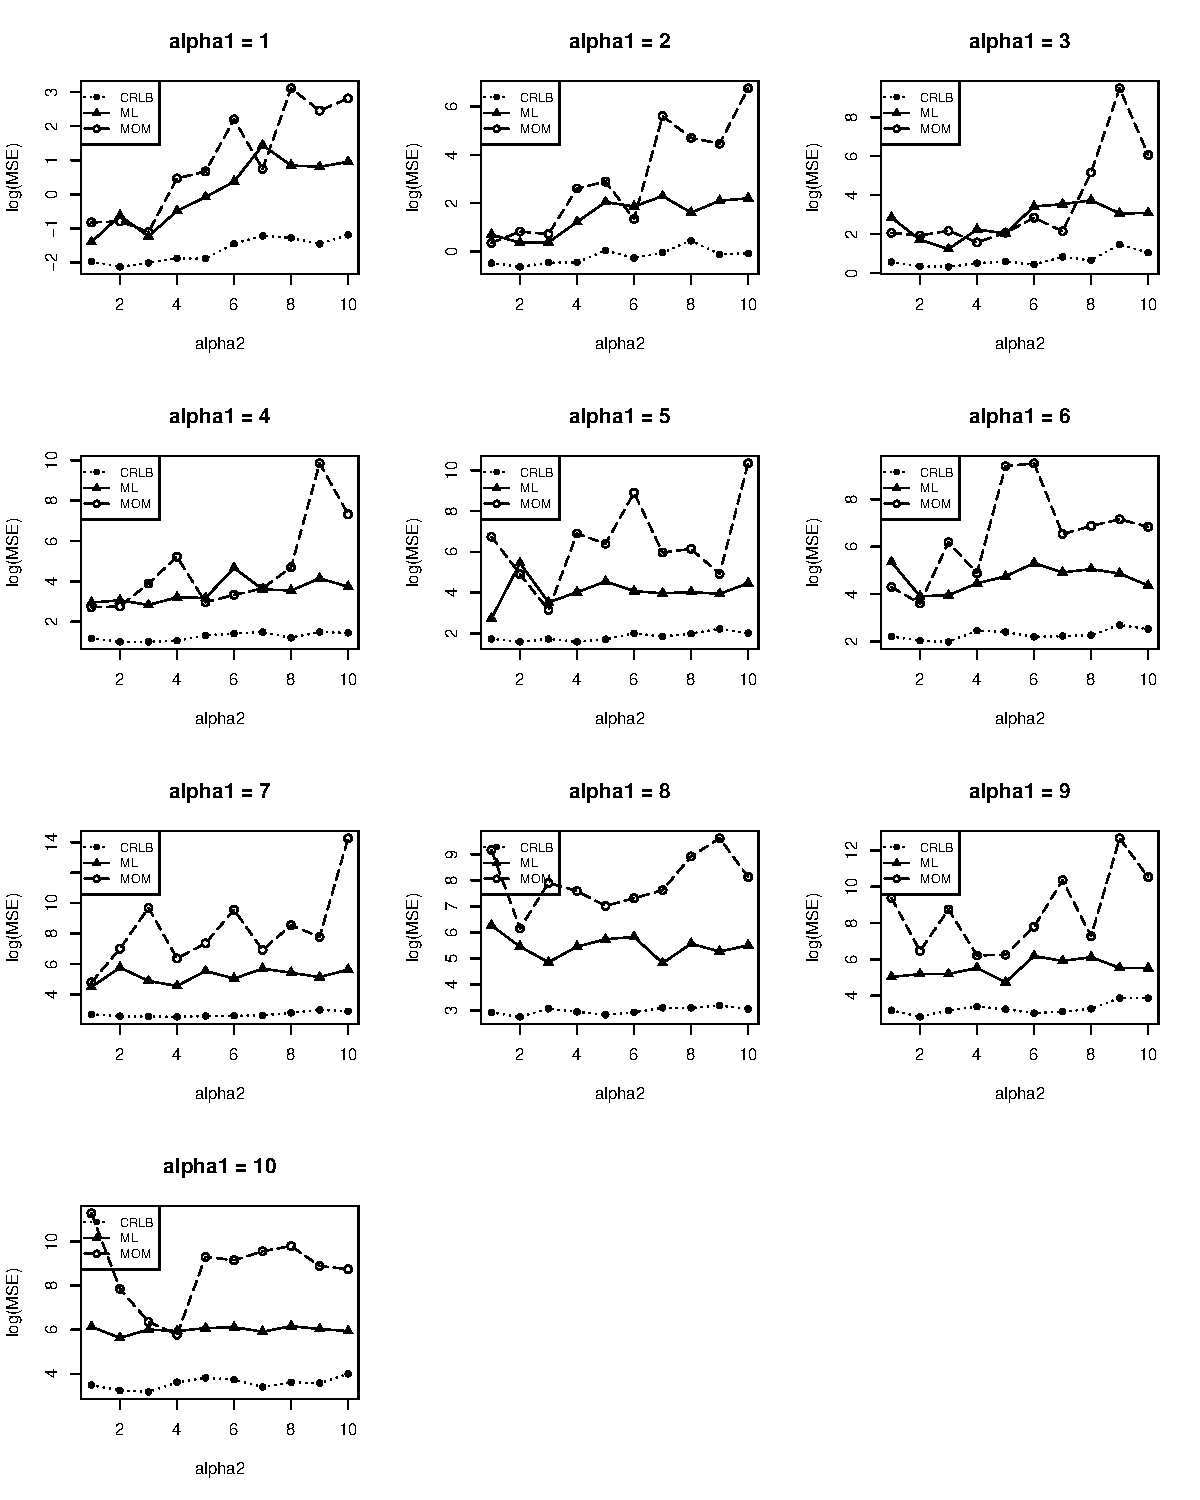
\includepdf{plot.pdf}

The graphs compare CRLB and the MSE of the two methods discussed above in logarithmic scale. In our experiment, we took 10 by 10 grid to generate the data sample from Beta binomial distribution. For each generated data we estimate the parameters for the beta binomial. These plots compare CRLB and MSE of ML and MOM for a given $\alpha_1$  to the range of $\alpha_2$. The x-axis shows the range of $\alpha_2$ corresponding to the MSE on the y-axis.\\
\\ 
The result shows CRLB has the smallest value compared to all estimation methods for all experiments. Our empirical result agrees to the analytical explanation of CRLB, which claims CRLB is the lowest bound for MSE of any estimator. Furthermore, the lower bound variance for the examples generated from larger $\alpha_k$ parameters tends to have bigger value compared to data generated from smaller parameters.\\
\\
In the other hand, MLE achieves lower MSE than MOM  for most examples generated. However, in few experiments there exist a situation where MOM beats MLE. For example, we can see some points in the plots of $\alpha_1$ less than 6 where MOM has smaller MSE value than MLE. Analytically, we expect MLE to outperform MOM for large sample size as MLE is asymptotically efficient. However, in the smaller sample size dataset there could be a situation where MOM could beat MLE . The result of some plot in our experiment shows MOM could also achieve better estimation than MLE. This is because our experiments is based on small sample size (i.e. m=20 document size).
\begin{thebibliography}{9}

\bibitem{minka}
Thomas P. Minka.
\newblock Estimating a Dirichlet distribution.
\newblock 2012.
\bibitem{Guo76}
 B.N. Guo and F. Qi, 
\newblock Inequalities and Monotonicity for the Ratio of Gamma Functions,
\newblock Taiwanese Journal of Mathematics, 
\newblock Vol 19, No. 7. pp. 407-409. (1976).
\end{thebibliography}

\end{document}
